%%%%%%%%%%%%%%%%%%%%%%%%%%%%%%%%%%%%%%%%%%
\chapter{Literature Review}\label{sec: literature}
\markboth{}{Literature Review}
\epigraph{\emph{}}{\citep[]{bilbow2022}}

This literature review takes a retrospective view at the history of augmented reality technologies. In laying clear the origination of these technologies within predominantly visual fields of research, it allows for a critique of preconceived notions about the definitions of what AR is, and the boundaries of how it is used today. The review outlines the contemporary forms, sensory display techniques, and methods taken to mediate our reality with virtual processes. In sketching out this wide variety of possible arising interactions, I make clear the benefit of considering AR as a medium for expressive computational artwork, namely in its inherent ability to approach technology from a creative and inclusive perspective (not just from the perspective of viewing AR as a visual overlay tool). I then touch on examples of AR art that make much more creative use of the materiality of AR in this way.



%%%%%%%%%%%%%%%%%%%%%%%%%%%%%%%%%%%%%%%%%%
\section{The Augmented Reality Interface}\label{sec: literature-interface}
\subsection{History of AR}\label{sec: literature-interface-history}
The earliest conceptions of what we would today call AR began their development in 1965 with Ivan Sutherland's `Ultimate Display' \citeyearpar{sutherland1968}. Sutherland's project involved hypothesising and developing a computer interface that could serve `as many senses as possible'. He speculated that this interface could `serve as a looking-glass into the mathematical wonderland constructed in computer memory'. By 1968, Sutherland had constructed what he called a `head-mounted three dimensional display', with a which was affixed to the ceiling of his lab with mechanical tracking arm that measured the position and orientation of the display in the room, called `The Sword of Damocles'. The head-mounted display provided per-eye visual displays via mini-CRT monitors, whose content was updated in real-time, dependent on the tracked pose of the head. This resulted in the three-dimensional (visual) perception of a hybridised real and virtual space, see \autoref{fig: sutherlandsword}.

\begin{figure}[bth]
    \myfloatalign
    {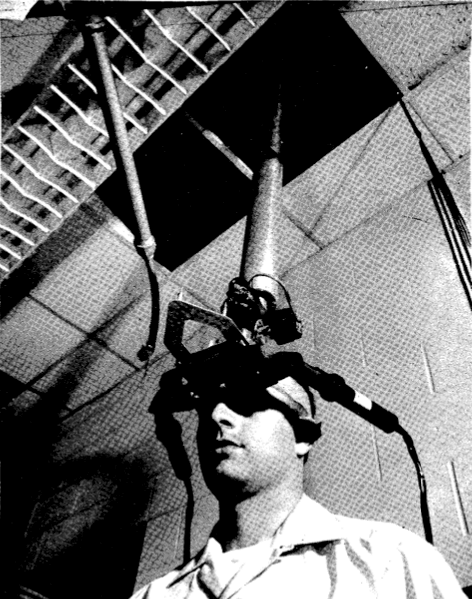
\includegraphics[width=.45\linewidth]{c_2/sutherland68_2.png}}
    \caption[Sutherland's `Ultimate Display']{Sutherland's `Ultimate Display'}\label{fig: sutherlandsword}
\end{figure}

Over the course of the proceeding thirty years, most display (visual, audio and haptic) technologies gained higher resolutions, whilst becoming ever more miniaturised, propelled by the general movement towards ubiquitous and wearable computing.  In 1992, augmented reality (AR) was officially defined by Boeing engineers Thomas Caudell and David Mizell, as a technology that could be used to `augment the visual field of the user with information' \citeyearpar{caudell1992}. Their prototype device featured display and tracking technologies built on the work of Sutherland. The purpose of the Caudell and Mizell’s device was to increase manufacture workers' efficiency through overlay of graphical wireframe instructions. Their device operated by tracking elements of the users environment and body, processing these in real-time, and then overlaying these instructions in the appropriate places dependent on the manufacturing process through a HUDset. The HUDset, commonly referred to today as a head-mounted display (HMD) operated by updating the displays output in real-time dependent on the position and orientation (pose) of the participant. This had the effect of the graphical overlay seeming `fixed', or what is referred to now as `registered' or `aligned', on top of a specific point in the real world. For Caudell and Mizell, this display and tracking solution is what leads to the `technology' of AR being possible, and for them, it is what enables the context-aware instructional overlay of their application.

\begin{figure}[bth]
    \myfloatalign
    {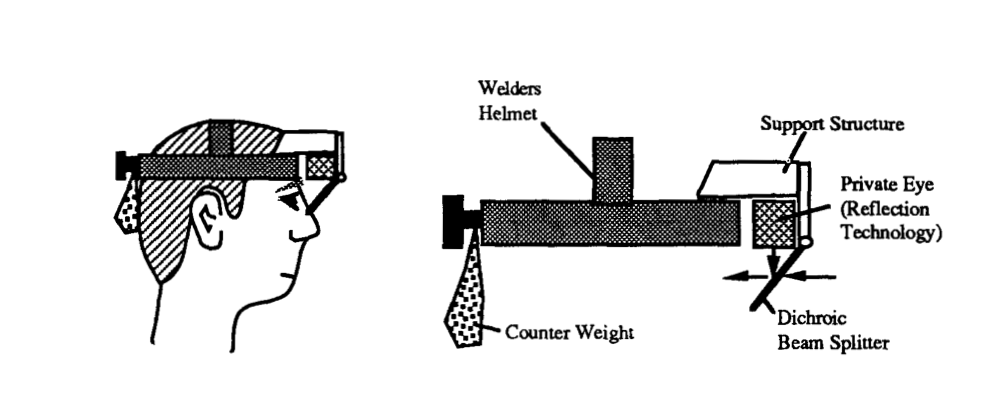
\includegraphics[width=0.75\linewidth]{c_2/caudell92_1.png}}
    \caption[Caudell and Mizell's device]{Caudell and Mizell's device}\label{fig: caudellprivateeye}
\end{figure}

Shortly after this original definition, Milgram and Kishino conceptualised the `Reality-Virtuality Continuum \citeyearpar{milgram1994}, which aimed to consolidate similar efforts across disciplines that were aiming to augment or virtualise `reality'. The continuum (\autoref{fig: milgramcontinuum}) defines two outer bounds of `Real Environments' on the left (which exist as physical and tangible matter), and `Virtual Environments' on the right (that exist solely as digital bits), and everything within was to be classed as `Mixed Reality' (MR). Within MR, use-cases closer to the `Real' were regarded as `Augmented Reality' (AR), and use-cases closer to the `Virtual', were regarded as `Augmented Virtuality' (AV). In separating these MR use-cases from the tele-robotics field of Virtual Reality / Virtual Environments (VR / VE), they proposed a clear framework for classifying works. Since both AR and AV make use of augmenting `by means of real objects' in today's use cases, (e.g. by tracking and parameterising hand gestures, or tracking and generating spatial maps of the real environment), the difference between AR and AV in this definition, problematically, becomes the `primary world' in which objects are are doing the augmenting. Indeed, Milgram and Kishino make note of the possibility of this in their paper: 

\begin{figure}[bth]
    \myfloatalign
    {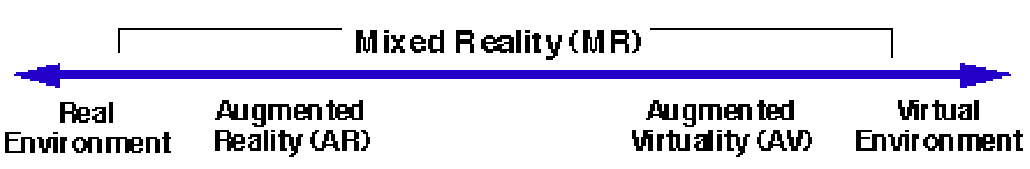
\includegraphics[width=0.75\linewidth]{c_2/milgram94_1.png}}
    \caption[`Reality - Virtuality Continuum']{`Reality - Virtuality Continuum'}\label{fig: milgramcontinuum}
\end{figure}

`Of course, as technology progresses, it may eventually become less straightforward to perceive whether the primary world being experienced is in fact predominantly `real' or predominantly `virtual', which may ultimately weaken the case for use of both AR and AV terms'

They further specify that, despite this is the case, it should not affect the validity of the more general [Mixed Reality] term to cover the `grey area' in the centre of the virtuality continuum, and also offer the term `Hybrid Reality' for displays that blend AR and AV compositely. Today, term `Mixed Reality' is seen seldom apart from its use within Microsoft's toolkit, and `Hybrid Reality' even less so. Therefore, as previously mentioned, due to the rapid evolution of these technologies, the present thesis makes no distinction between Mixed, Hybrid, and Augmented Reality.

In 1997, Azuma proposed a specification for the definition of an AR system, and surveyed the five years of AR research since Caudell and Mizell's original definition. In order to avoid limiting AR to specific technologies, they define AR as a `system' that follows three characteristics: 

\begin{itemize}
    \item Combines real and virtual
    \item Interactive in real time
    \item Registered in 3-D
\end{itemize}

In this paper, he distinguishes between optical and video based approaches to AR and while both of these methods can and had been realised (when speaking strictly of visual display of information) via head mounted display technologies, Azuma makes further room in the definition for monitor based approaches too, allowing the definition to be broad enough to encompass a variety of AR use cases, methods and processes. Not soon after, Azuma et al., classify three categories of `display': head worn, handheld and projective. For this reason, as well as the specification of three precise characteristics, Azuma’s definition of AR has become widespread. 

These early definitions and conceptions of AR were typically built upon with applications involving display and tracking technology that resulted in the \textbf{visual overlay and alignment} of \textbf{virtual graphics} onto our \textbf{real world environment}. Whilst this view of AR is followed by the overwhelming majority of historical and contemporary uses of AR, it only makes up a small subset of the potential myriad interactions afforded by the technologies that enable AR. Sutherland, who arguably catalysed early practical research in this field, viewed this AR as a `window' interface, that could serve `as many senses as possible'. Rosenberg, another early proponent of AR, developed the concept of `Virtual Fixtures' (overlaid sensory information) as a method of reducing the `tax' on our senses induced by an overload of information through the visual sense \citep{rosenberg1993}. Milgram and Kishino, in outlining their taxonomy, recognise that it could serve to alleviate `analogous issues associated with other display modalities`, and cite work from Cohen, who at the time was developing realistic acoustic environment rendering in AR \citeyearpar{cohen1993}. They also note the concurrent work in haptic (the various senses of touch) displays for augmented reality. 

Mann terms `Mediated Reality' \citeyearpar{mann1994} as more of a method to computationally mediate our own perception, rather than just focusing on overlaying. His later work terms `All Reality (*R)' which broadens the taxonomy of AR with concepts such as as surveillance and privacy \citeyearpar{mann2018}. Azuma et al., acknowledge that AR is not just limited to visual perception or overlaying processes: `AR can potentially apply to all senses, including hearing, touch, and smell. Certain AR applications also require removing real objects from the perceived environment, in addition to adding virtual objects'. With this in mind, what does the landscape of more contemporary AR design look and feel like today?



\subsection{Forms of AR}\label{sec: literature-interface-forms}
\subsubsection{Head-mounted}\label{sec: literature-interface-forms-hmd}
\begin{figure}
    \centering
    \subcaptionbox{Sutherlands `Ultimate Display'\label{fig: historicalHMDs-sutherland}}[.3\linewidth]{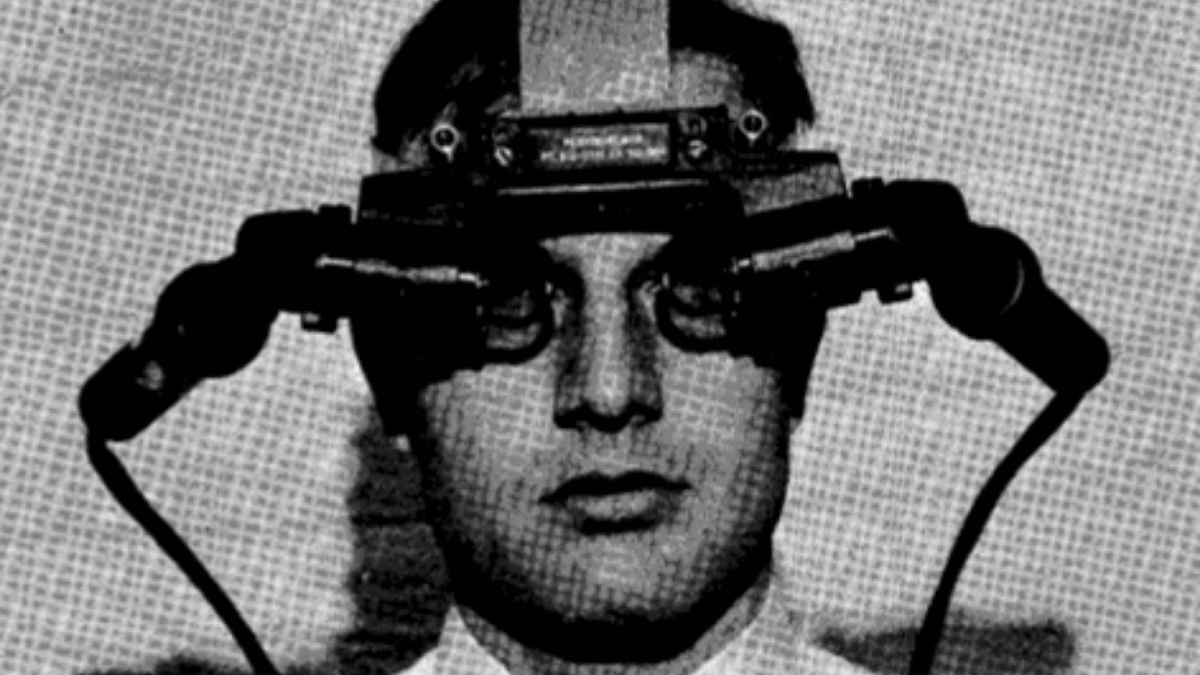
\includegraphics[height=2.5cm]{c_2/sutherland68_1.png}}
    \hfill
    \subcaptionbox{Caudell and Mizell's `HUDset'\label{fig: historicalHMDs-caudell}}[.3\linewidth]{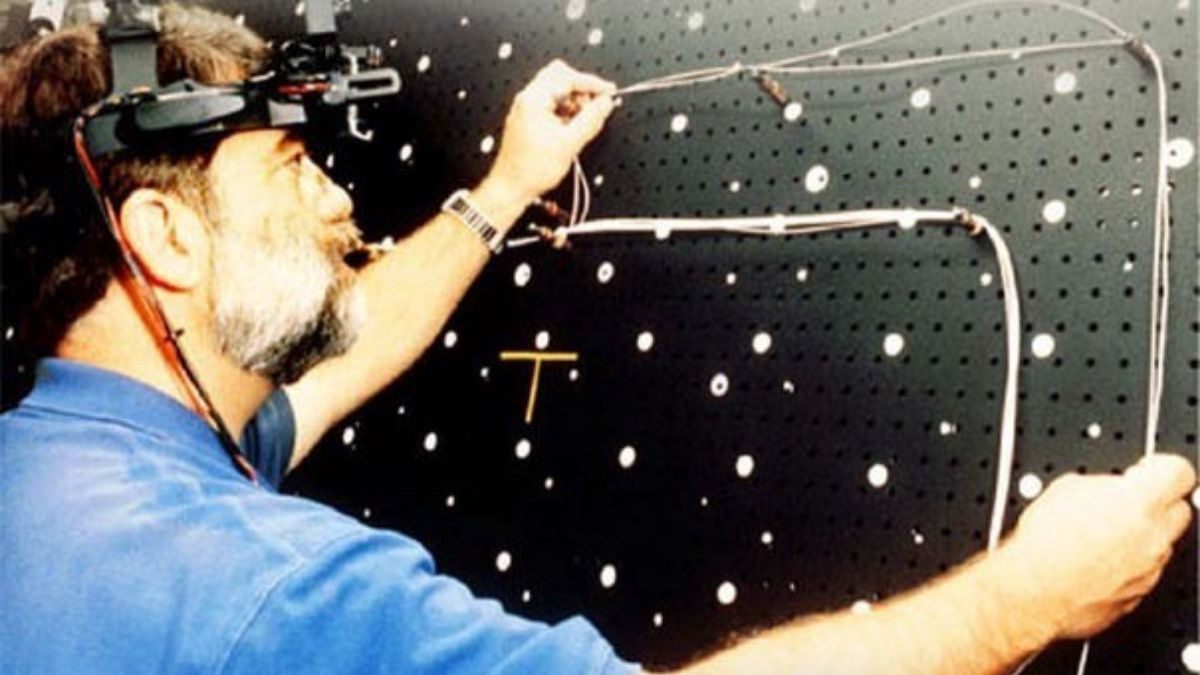
\includegraphics[height=2.5cm]{c_2/caudell92_2.jpeg}}
    \hfill
    \subcaptionbox{Feiner's `KARMA' System\label{fig: historicalHMDs-feiner}}[.3\linewidth]{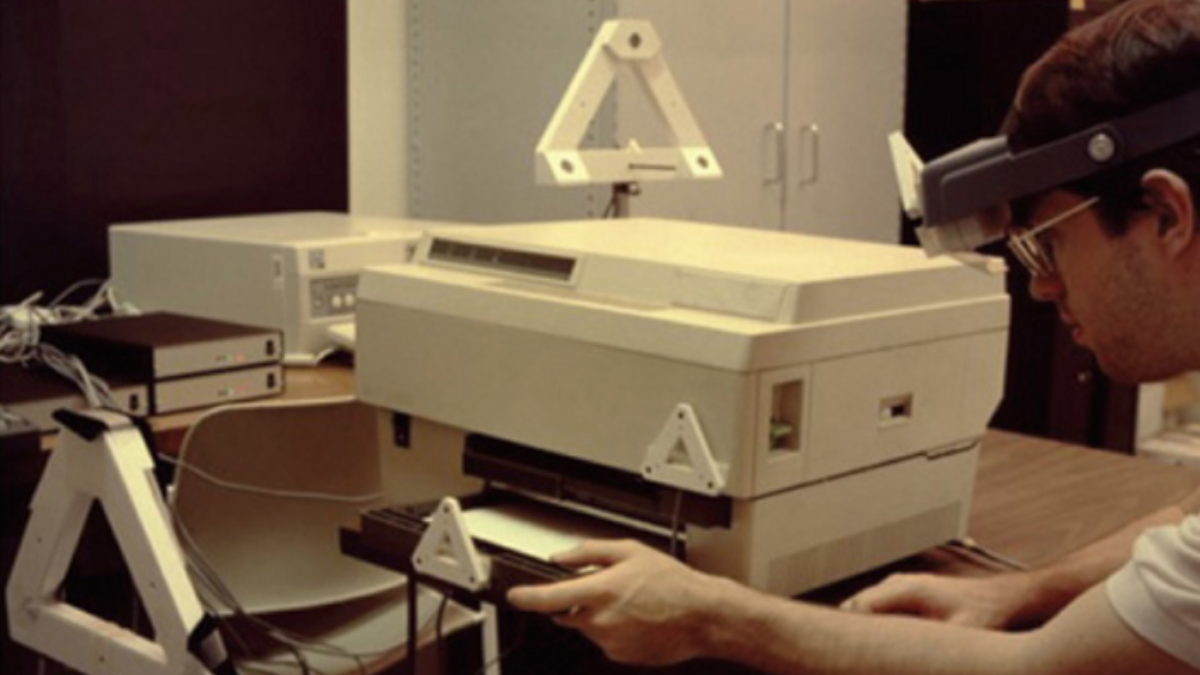
\includegraphics[height=2.5cm]{c_2/feiner93_1.png}}%
    \caption{Historical AR HMDs}
    \label{fig: historicalHMDs}
\end{figure}

Successors of AR head-mounted displays (HMDs) devised by Sutherland \citeyearpar{sutherland1968}, Caudell and Mizell \citeyearpar{caudell1992}, and Feiner \citeyearpar{feiner1993,feiner1997} exist today commercially within products such as the Microsoft Hololens 2 \footnote{\url{https://www.microsoft.com/en-us/hololens}}, the Magic Leap ML-1 \footnote{\url{https://www.magicleap.com/magic-leap-1}}, and the nReal Light \footnote{\url{https://nreal.ai/product/}}. These devices afford optical see-through capabilities through half-mirror visors and high-resolution displays, and offer stereo audio output. Input is managed mainly by hand-tracked interaction with overlaid visual menus and objects, but is also possible through eye tracking and voice control. The environment is sensed through a combination of 6DoF pose tracking, and spatial mesh mapping. For most HMDs today, this input and environment processing occurs off-device, on a tethered or wearable computer, or mobile device. These devices tend to be relatively expensive due to the extremely high R\&D costs associated with the field (due to its novelty). Leap Motion's open-source Project North Star \footnote{\url{https://docs.projectnorthstar.org/}} provides a much cheaper alternative at the trade-off of slightly larger form and lack of integrated computing and audi o implementation, but has the highest field-of-view of all four and comparable tracking.

\begin{figure}
    \centering
    \subcaptionbox{Microsoft Hololens 2\label{fig: contemporaryHMDs-microsoft}}{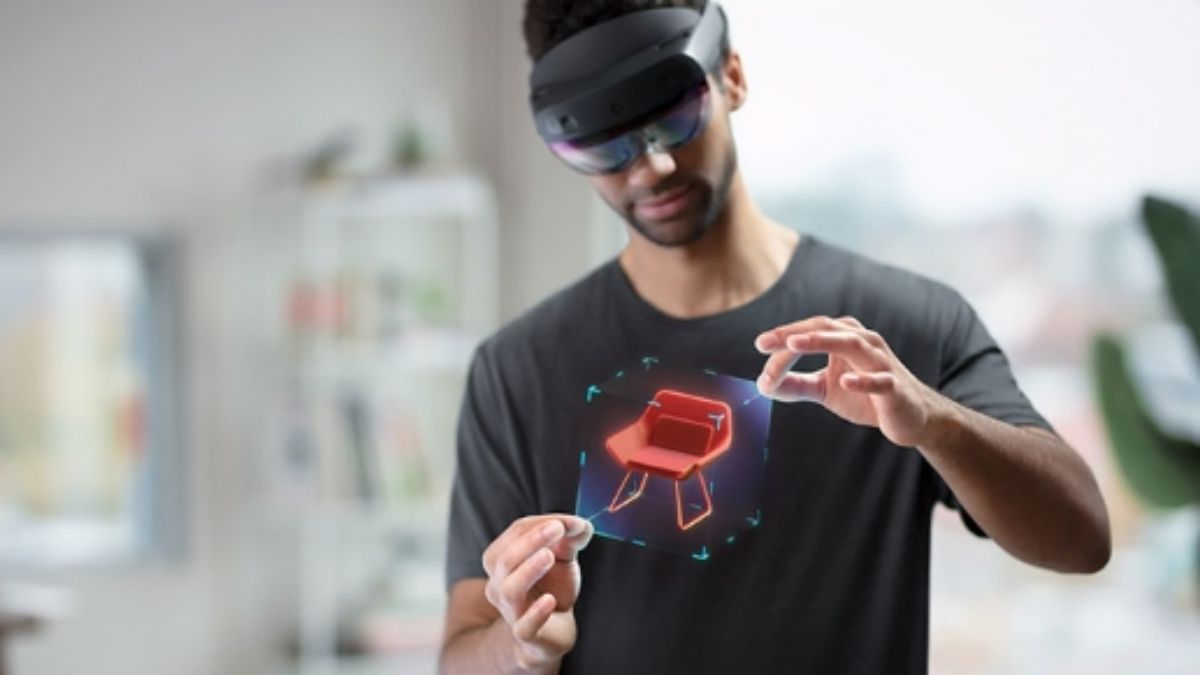
\includegraphics[width=0.45\linewidth]{c_2/hololens.jpg}}\quad
    \hfill
    \subcaptionbox{Magic Leap ML-1\label{fig: contemporaryHMDs-magicleap}}{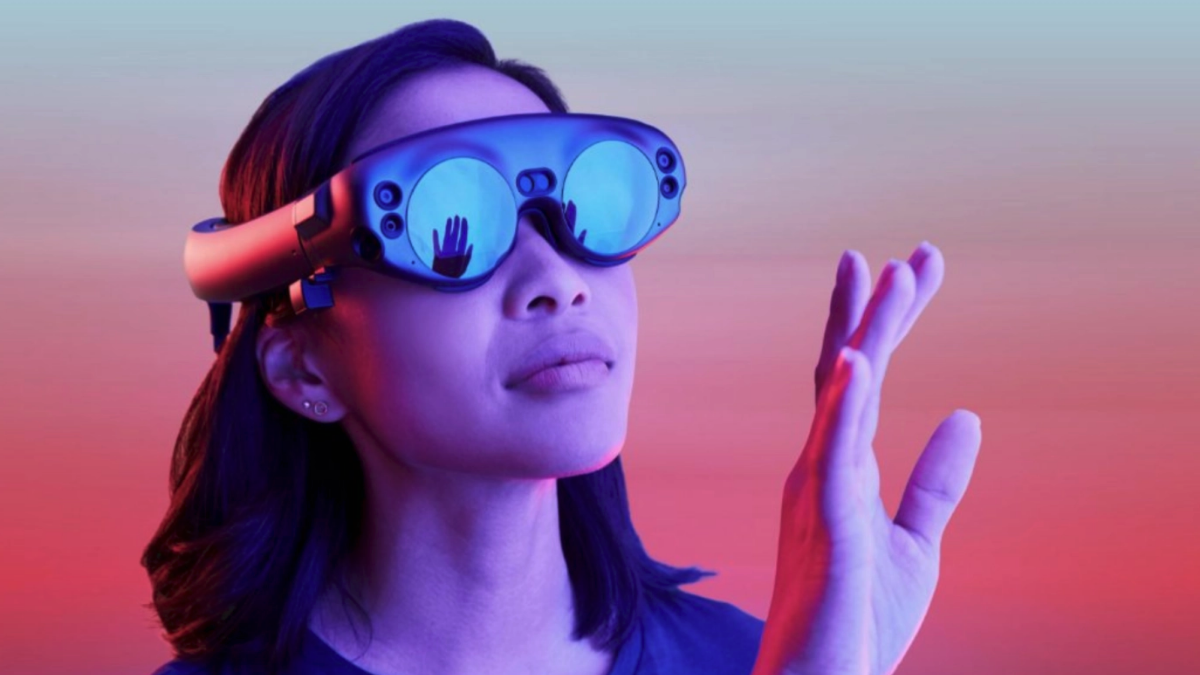
\includegraphics[width=0.45\linewidth]{c_2/magicleap.png}}\\
    \vspace{0.5cm}
    \subcaptionbox{nReal Light\label{fig: contemporaryHMDs-nreal}}{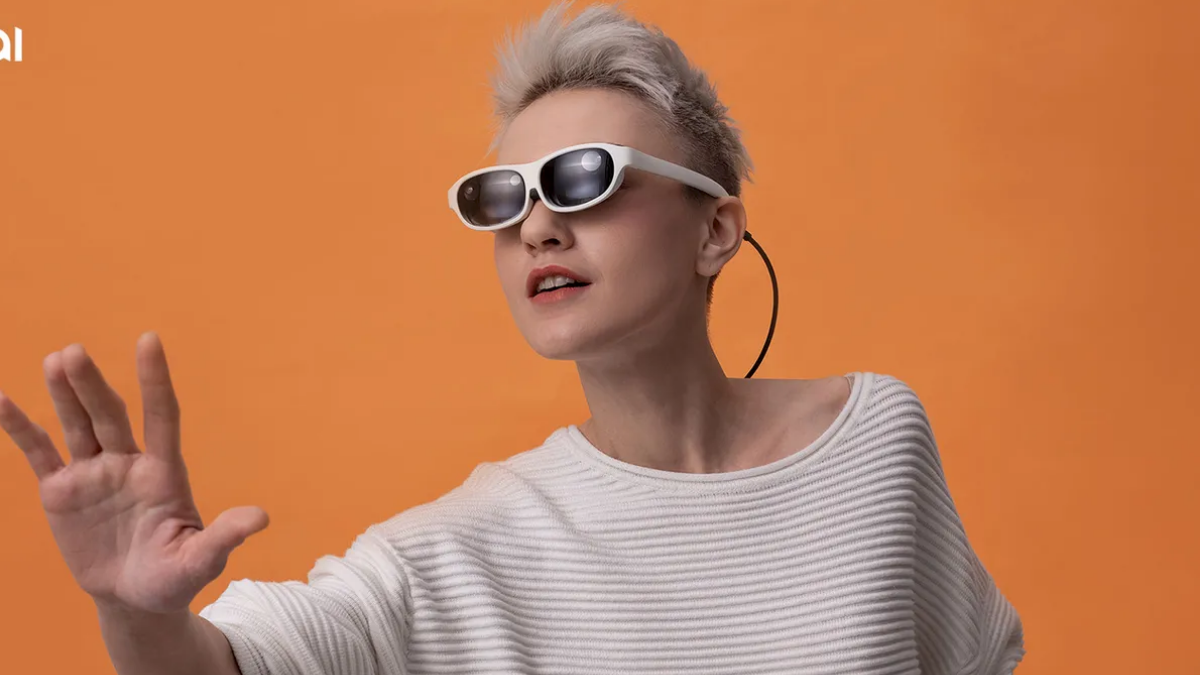
\includegraphics[width=0.45\linewidth]{c_2/nreal.png}}\quad
    \hfill
    \subcaptionbox{Leap Motion Project North Star\label{fig: contemporaryHMDs-northstar}}{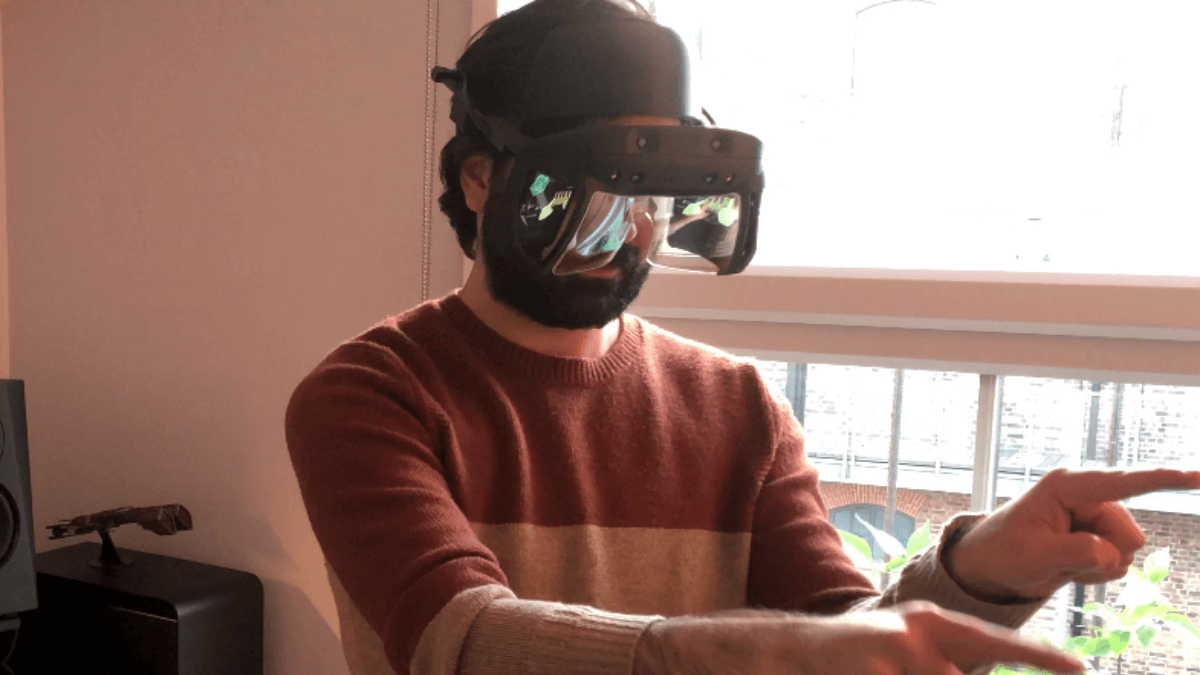
\includegraphics[width=0.45\linewidth]{c_2/northstar.png}}\\
    \caption{Contemporary AR HMDs}
    \label{fig: contemporaryHMDs}
\end{figure}

A device that is head-mounted poses clear benefits to both input and output modalities. For input sensors, being mounted on the head provides them with more accurate tracking from the perspectives of our own senses (organic sensors).  Consequently, and as Lindeman and Noma maintain in their classification scheme for multisensory AR, an important factor for the parity (if desired) of real and virtual output is a consideration of the location along the `stimulus pathway' at which they mix: at the environment, sensory subsystem or computer level \citeyearpar{lindeman2007}. For a device to be head-mounted, allows `mixing' to happen closer to the sensory subsystems, i.e. our eyes, ears, nose and mouth, thus resulting in an experience that is more closely intertwined with our real-time environment stimuli.

\subsubsection{Handheld}\label{sec: literature-interface-forms-mobile}
Today, anyone who owns a smartphone is carrying an AR device in their pocket. This particular genre of AR development began in earnest in the mid 2000's and today is the most widely used form of AR due to the pervasiveness of smartphones. It builds on the early research and practice of handheld AR applications built on cellphones and personal digital assistants (PDAs) in the late 1990's, and smartphones in the late 2000’s, whose increasing variety and accuracy of onboard sensors: cameras, gyroscopes, accelerometers, and GPS, provided a convenient all-in-one solutions for developing handheld visual AR experiences. 

The limitations of handheld displays are outlined by Bimber and Raskar \citeyearpar[pp. 79-83]{bimber2005}: reduced immersiveness due to the small screen size, compounded by the distance between it and the participant (normally arms length), impaired gestural input due to the need to hold the device; restrictions due to the cameras image quality and less computational power available to effectively register (align) real and virtual objects. As well as these issues, smartphones have developed to be primarily visual devices despite their name, and as such, their ability to deliver high fidelity audio, let alone audio AR mixing is limited due to their distance from the ear. 

Recently, the lack of non-visual AR in handheld smartphones has been addressed through the increased adoption of `hearables', a marketing term for small and unobtrusive, wireless earphones. More specifically, two features make these suitable audio solutions for AR use; `transparent' hearing modes (see mic-through \citep{lindeman2008}), and integrated 6DoF \footnote{\url{https://www.apple.com/airpods-pro/specs/}}.

\subsubsection{Projective}\label{sec: literature-interface-forms-proj}
Projection of data into the environment in order to overlay or alter perception of real objects, i.e mixing virtual and real stimuli at the environment level \citep{lindeman2007}, is perhaps the least adopted of Azuma's categories of AR. The property that sets projective AR apart from head-mounted and handheld AR is perhaps its potential to deliver experience to multiple participants within a space. Although collaboration is possible through the previous two categories, it requires all participants to engage technology that is affixed to their body (either through wearing or through holding). Projective AR alleviates both the burden of physical attachment to a device, and also the expense of procuring a device for each participant. This category of display is typically realised by use of video projectors and speakers. Although the base requirement of registration in three-dimensions between virtual and real (Azuma's third specification), is fulfilled relatively easily (add more projectors) compared to head-worn and handheld approaches (more sensor computation and accuracy), 

\subsubsection{Other forms}\label{sec: literature-interface-forms-other}
Of course, this categorisation is not exhaustive, and leaves out body worn AR systems such as the Audiomented Sound System \citep{chevalier2020}, and tangible augmented objects \citep{schraffenberger2015}. This will be expanded on within my own framework towards designing multisensory AR instruments.



\subsection{Sensory Display in AR}\label{sec: literature-interface-sensory}
Within these common forms of AR technology, one could split the various technological processes that occur into input, process, output (the general IPO model found in software engineering), in AR this is often labelled: tracking, process, display. Tracking, as mentioned is often through hand gesture, body position and orientation and voice activation. Display is managed in the majority of cases through screens. The present section outlines various other sensory displays that have the potential of creating more immersive tools of expression.

\subsubsection{Visual Sense}\label{sec: literature-interface-sensory-visual}
It is poignant to mention that until that last 20 years or so, sensory sciences, and as a result, technological displays of information, were focused on the visual, with the auditory following behind, and then the touch, smell and taste senses. In cross-modality psychology research, this ocular-centrism (the perceptual and epistemological bias ranking vision over other senses) is normally explained by a `textbook' explanation: `the idea that vision is the most important modality is supported by numerous studies demonstrating visual dominance.' Fabian Hutmacher argues that ocular-centrism can be critiqued through the lenses of \citeyearpar{hutmacher2019}: 

\begin{itemize}
    \item A methodological-structural explanation: `Research on vision is often easier than research on other modalities and that this is the result of an initial bias toward vision that reinforces itself.'
    \item A cultural explanation: `The dominance of the visual is not a historical constant, but rather a result of the way (Western) societies are designed.'
\end{itemize}

However, AR is still typically realised in the form of graphical overlay, and as such, the forms which we find ourselves interacting with are predominantly based around screens and other forms of visual display \citep{dey2018}. These are often split into optical and video see-through methods of display. The former employs semi-reflective half-mirrors to combine the reflection of close-by screen with the natural pass-through of the real world; the latter uses the feed of cameras to completely occlude the participant's vision, and performs AR processes on top of the camera feed. There are advantages and disadvantages to both methods, outlined in \citep{rolland2000}. Head-mounted systems tend towards optical see-through, whereas most handheld AR (smartphones) are exhibit video see-through AR.

\subsubsection{Auditory Sense}\label{sec: literature-interface-sensory-auditory}
The second most developed-for sense in AR is the auditory system, borrowing from a rich history of spatial audio techniques such as exploiting HRTF for binaural audio playback and realistic audio localisation. Within the field of audio AR, as previously mentioned, `hearables' with `transparency hearing` modes offer the auditory equivalent of video see-through (coined mic-through \citep{lindeman2008}), where the occluded outside world is captured through a microphone, on top of which virtual sounds can be processed. Also outlined by Lindeman and Noma is the use of bone conduction headphones to offer a mediated perception of sound environments without the need to occlude the participants ears (coined hear-through), which could be considered equivalent to optical see-through. Moving into the environment, there are a myriad spatial audio techniques that could be used within AR, delivered by speaker arrays such as those found in wave-field synthesis and ambisonic beam-forming practices.

\subsubsection{Haptic Sense}\label{sec: literature-interface-sensory-haptic}
Due to the prevalence of hand-tracking technologies in the interaction with head-mounted AR applications, one might assume that being able to actually \emph{feel} the virtual objects that are placed in AR would be one of the most important and developed concepts in AR. However, much of the early research in AR placed importance around overlaying instructions, rather than interactive objects. Hence, the haptic feedback of touching AR objects is relatively under-explored compared to the common issues which affected early and (funded) research - accurate registration of real and virtual processes; and higher visual fidelity. In most cases, it was deemed enough to \emph{see} the effect that ones hands or body position had on the AR object or scene respectively. Today, there exist numerous technologies that could provide computationally mediated haptic perception in AR, for example through vibrotactile feedback or electrical muscle stimulation \citep{lopes2018}.

\subsubsection{The Chemical Senses}\label{sec: literature-interface-sensory-chemical}
Whereas auditory and haptic sensations have been developed in AR, the chemical senses (smell and taste) have received far less exploration. Visual, auditory, and touch information can be believably recreated with technology through analog to digital conversion of electromagnetic radiation (light) and mechanical wave transmission (sound and touch). Conversely, smells and tastes contain organic information, the sensors (and thus A2D conversion) for which have not been invented yet. As such, the closest we can get to receiving chemical sensory data is through computationally activated rather than computationally mediated displays: scent emitters \citep{maggioni2019}, and taste patches for example. Accordingly, in order to mediate the sense of taste, creative methods of sensory illusion have often been employed, i.e. Narumi et al. demonstrating that the sense of flavour can be mediated via visual overlay in AR \citep{narumi2011}. The sense of temperature has also been mediated through cross-modal sensory illusion exploiting the trigeminal nerve in the nose, Brooks et al. demonstrates that users in VR can be made to feel warmer or colder based on the relative amounts of capsaicin or eucalyptus emitted near the nose \citeyearpar{brooks2020}.


\subsection{Computationally Mediated Realities: The AR Process}\label{sec: literature-interface-process}
Additive layering of virtual content onto our real environment is by far the most typical of processes experienced in AR. However, it is only one of the potential methods of interaction between virtual and real components. In navigating this issue, the present thesis aligns its conception of AR closely with the definition of AR by Chevalier and Kiefer \citeyearpar{chevalier2020}: `real-time computationally mediated perception', which fulfils Azuma's three characteristics of AR systems, but is not as exclusionary as Caudell and Mizell's original definition: a technology used to  `augment the visual field of the user with information'. Investigating the existing relationships between real and virtual components of AR systems, Schraffenberger outlines at least five `relationships' and five `subforms' of AR (see \autoref{table:schraffenbergertaxonomy}). This taxonomy \citeyearpar[pp. 80-130]{schraffenberger2018} provides an ideal starting point for those designing AR systems interested in creating embodied experiences that challenge the typicality of basic visual-overlay AR. Furthermore, Mann expands the `Reality - Virtuality Continuum' \citep{milgram1994} into the `All Reality Continuum', integrating further dimensions such as `Metaveillance', `Kineveillance' and `Phenomenality', such a standpoint not only `anticipates the need for an ethically aligned reality' \citeyearpar{mann2018}, but demonstrates the multifaceted nature of augmented reality to afford experiences of ourselves, others, and environments computationally mediated by more than just additive informational overlays.

\begin{table}
    \centering
    \begin{tabular}{ l l }
        \toprule
        Relationship        & Description                       \\
        \midrule
        Coexistence         & Unrelated                         \\
        Presence            & Spatially Related                 \\
        Information         & Content-Based Relationship        \\
        Physical            & Affect Each Other                 \\
        Behavioural         & Sense and React to Each Other     \\
        \midrule
        \midrule
        Subform             & Description                       \\
        \midrule
        Extended Reality    & The Virtual Supplements the Real  \\
        Diminished Reality  & The Virtual Removes the Real      \\
        Altered Reality     & The Virtual Transforms the Real   \\
        Hybrid Reality      & The Virtual Completes the Real    \\
        Extended Perception & Translating the Inperceptible     \\
        \bottomrule
    \end{tabular}
    \caption{Schraffenberger's taxonomy of relationships and emergent AR subforms}\label{table:schraffenbergertaxonomy}
\end{table}

In particular, `diminished reality', aims to \emph{remove} real objects in our environment. When explored in the visual sense, this approach uses computer vision and content-aware substitution to remove a section or object of the real-world environment through camera sensors. Noise cancelling potentially offers an auditory diminished reality, but due to the fact that sound is propagated via mechanical waves, our sense of sound is closely intertwined with physically feelings of vibration, which are much harder to remove \citep{mori2017}. Further examples of sound-driven but cross-modal techniques are outlined in \citep{walther-hansen2020}.

`Altered reality' has the potential to provide new and otherwise inaccessible sensory and perceptual experience Schraffenberger describes that this is possible through virtual components altering the perception of real components in an AR system. Mann outlines a myriad examples of altered visual percepts \citeyearpar{mann1994}, from giants eyes, to `slow' glasses. More recently, Nishida et al. have experimented with `egocentric smaller-person experience' through use of a video see-through AR headset, in which unlike typical AR, the cameras are mounted at waist height, rather than on the HMD \citeyearpar{nishida2019}. This afforded participants a difference in real-time visual perception, and resulted in them generally feeling smaller and behaving more like a child. In tandem with this altered visual perception, they propose a modified robotic glove `HandMorph' \citeyearpar{nishida2020} that alters sensations of touch through reduced finger and overall grip size. 

\begin{figure}[bth]
    \myfloatalign
    {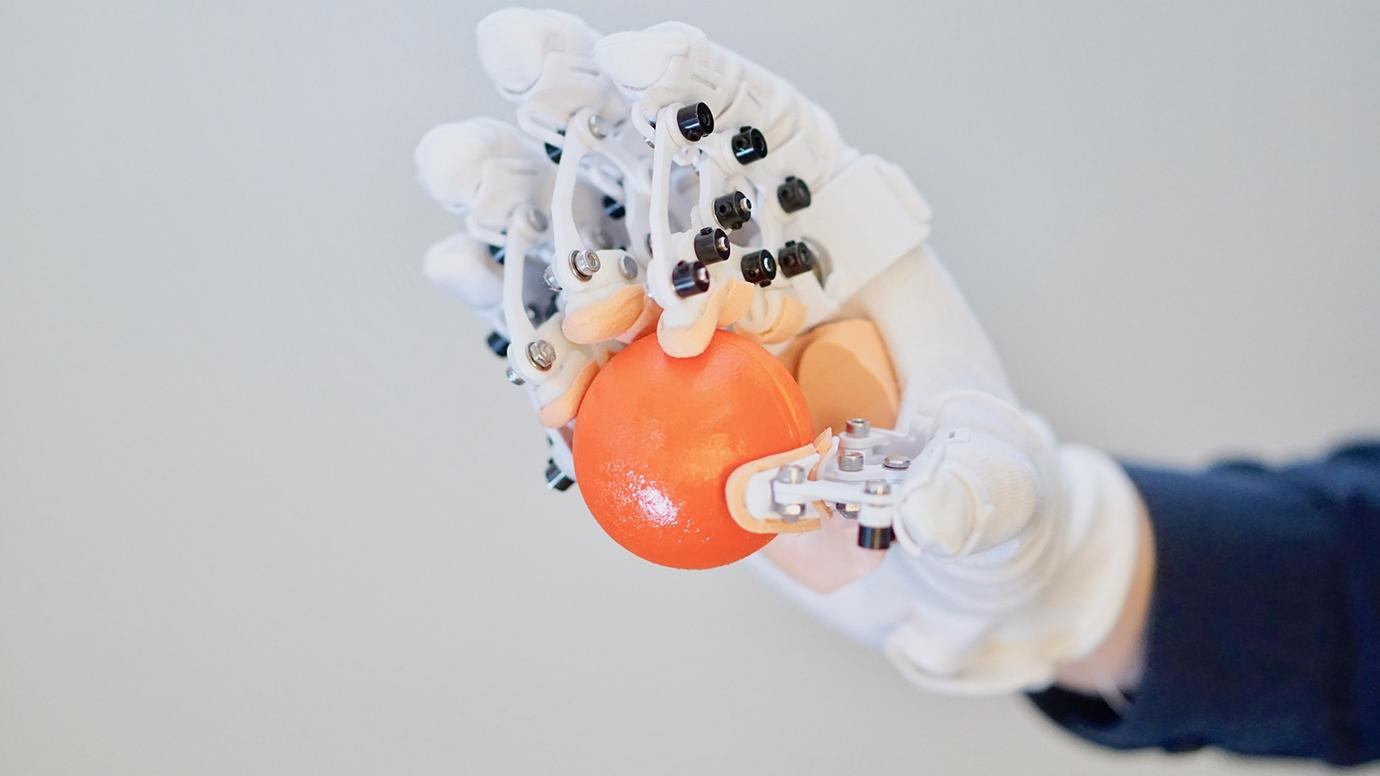
\includegraphics[width=.45\linewidth]{c_2/nishida20_1.jpg}}
    \caption[Nishida's `HandMorph']{Nishida's `HandMorph'}\label{fig: handmorph}
\end{figure}

In a similar vein, `extended perception' revolves around the potential to provide \emph{more} senses, or the sensing of stimuli outside of the range of our sensory systems. Bees for example have a visual system that extends far further into the ultraviolet range of EM radiation than our own eyes allow us; dogs hear much higher frequencies our ears allow us (thank goodness); and sharks can smell one part blood in a million parts water. These fun facts demonstrate vast differences in sensory acuity between species; but did you know that some shark have a constellation of pores \footnote{\url{https://www.sharktrust.org/shark-senses}} along the lateral side of their bodies that allows them to perceive minute pressure changes in water? This enables them to create a `pressure map' of their surroundings through active body movement. Modern technology could endow us with similar and myriad extended perceptions of our environment and its stimuli; Mann has experimented with making representations of radio waves translated down to the sensory range of our own eyes \citeyearpar{mann2018a}

\begin{figure}[bth]
    \myfloatalign
    {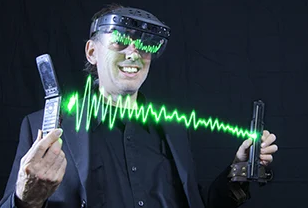
\includegraphics[width=.45\linewidth]{c_2/mann18_1.png}}
    \caption[Mann's `Sequential Wave Imprinting Machine']{Mann's `Sequential Wave Imprinting Machine'}\label{fig: mann_swim}
\end{figure}

 This section demonstrates the multitude of potential experiences that AR affords beyond mere visual information layering, next, I will examine the usage of AR in the arts, as a medium or tool for creating immersive aesthetic experiences, and demonstrate how this contributes towards a more holistic understanding of AR as a technology. 



%%%%%%%%%%%%%%%%%%%%%%%%%%%%%%%%%%%%%%%%%%
\section{Augmented Reality in the Arts}\label{sec: literature-arts}
Computational art, the use of computational programming or software as a tool, performance aid, medium or collaborator to create art or artistic works, is currently witnessing the adoption of new and exciting technologies such as trained machine learning algorithms, increasingly immersive displays and large-scale networked experiences. These implementations of technology within the creation artworks leads to a greater understanding of the materiality and affordance of these technologies. In this section, I draw attention the the modes of sensory engagment, aesthetic experience, collaborative expression, and activism that AR specifically affords artists willing to explioit its use as a medium.

\subsection{Sensory Engagement}\label{sec: literature-arts-sensory}
Computational art has seen the use of AR as a medium since the early 2000’s: in 2008, Grasset et al. presented case studies of AR art exhibitions, with the conclusion that for effective design of artworks, specific importance should be placed on the relationship \emph{between} real and virtual components \citeyearpar{grasset2008}. These relationships have come to describe a matrix of possibilities between senses and mediating processes, i.e. altered hearing, extended smell, diminished sight. Papagiannis has drawn attention to this broader multisensory view of AR in attempting to understand an aesthetic for AR applications, `AR is beginning to expand in new ways, beyond visual frames and into the full human sensorium' \citeyearpar{papagiannis2014}. In 2015, the Tate Sensorium multisensory art exhibition used novel mid-air haptic devices to augment visual art \citep{vi2017a}. The results of the included study found that more congruent multisensory experiences lead to audiences finding artwork more emotionally engaging. If more congruent multisensory experiences of art lead to more emotional engagement, and AR has the potential to mediate multiple senses in rich and provocative ways, surely this makes it an ideal medium for such works. 

\begin{figure}[bth]
    \myfloatalign
    {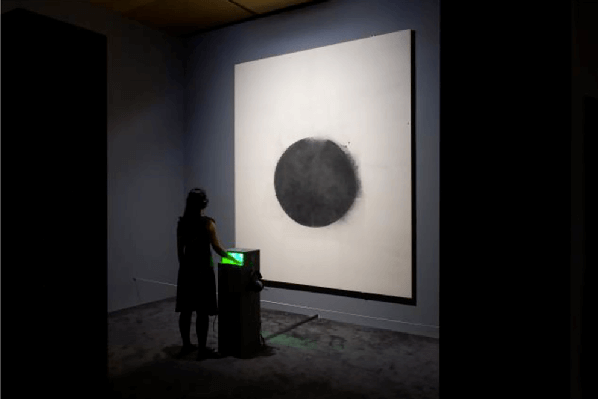
\includegraphics[width=.75\linewidth]{c_2/vi17_1.png}}
    \caption[Tate Sensorium Multisensory Art]{Tate Sensorium Multisensory Art}\label{fig: tate}
\end{figure}

\subsection{Aesthetic Experience}\label{sec: literature-arts-aesthetics}
Chevalier and Kiefer highlight the nascent use of newer AR technologies by artists \citeyearpar{chevalier2020}. They argue that AR has far more potential for creative exploration, and that it is a medium for creating `new nuanced and fine-grained emergent aesthetic experiences' and as previously mentioned, necessarily define AR as `real-time computationally mediated perception' in order to be inclusive of a multisensory approach to design. 

The installation `Concrete Storm'\footnote{\url{https://www.studiodrift.com/concrete-storm-microsoft}} by artists Gordijn and Nauta demonstrates the ability for AR to afford novel experiences of seemingly immutable and rigid physical objects (short concrete pillars), through the extension and animation of the concrete into larger, shifting and breaking structures. In describing the design of the work, they outline one of the main impetuses of creating the work: `Gordijn says the duo was interested in beginning to investigate the point at which viewers `might let go of trying to distinguish between what is real, what is not' and accept this new mixed world as simply another version of reality' \citep{gottschalk2017}. 

\begin{figure}[bth]
    \myfloatalign
    {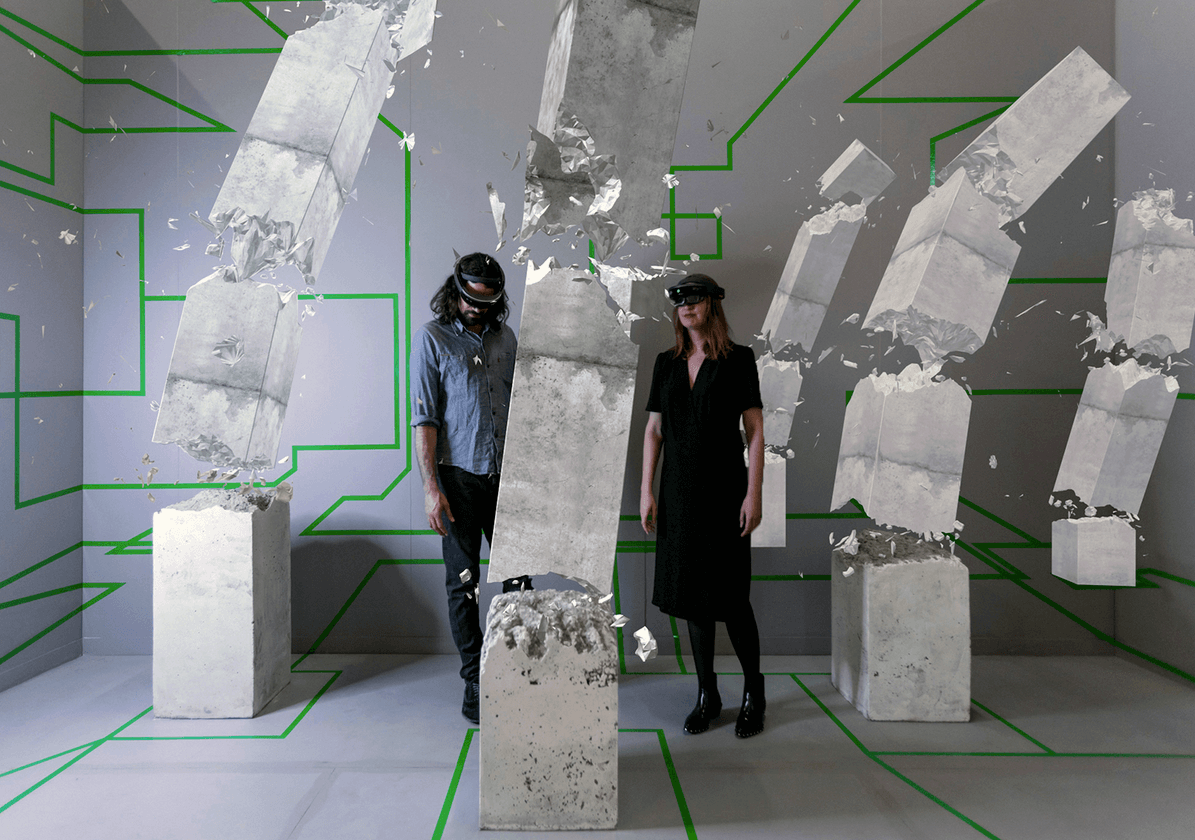
\includegraphics[width=.75\linewidth]{c_2/studiodrift.png}}
    \caption[Concrete Storm]{Concrete Storm}
\end{figure}\label{fig: concretestorm}

\subsection{Collaborative Expression}\label{sec: literature-arts-collaboration}
Another key aspect of the use of AR as a medium in computational artworks is its ability to enable collaborative expression and construct shared perceptual spaces. For example, Listening Mirrors\footnote{\url{http://listeningmirrors.net/}}, an artwork by Chevalier and Kiefer, \citeyearpar{chevalier2018} is an AR installation that engenders a collaborative and performative AR sound environment. This environment is hybrid in nature; split between physical and virtual space. In the installation space, participants can interact with a audio augmented parabolic acoustic mirror. Their interactions are intertwined with a computationally mediated virtual sonic environment that they experience through bone conduction headphones. Additionally their vocalisations are mediated by a wearable microphone through the mirror. This invites collaborative expression through exploration of the shared sonic world.

Similarly, Eno and Chilvers explore collaborative ambient audiovisual composition in their AR adaptation of the popular app `Bloom', `Bloom: Space' \footnote{\url{https://inculture.microsoft.com/musicxtech/bloom-open-space/}}. In this installation, participants wear a Microsoft Hololens and use hand gestures to activate and manipulate generative audiovisual elements. These elements can be experienced by other participants and thus create a shared perceptual and actionable space.

\begin{figure}
    \centering
    \subcaptionbox{Listening Mirrors\label{fig: collaborativeARt-listeningmirrors}}{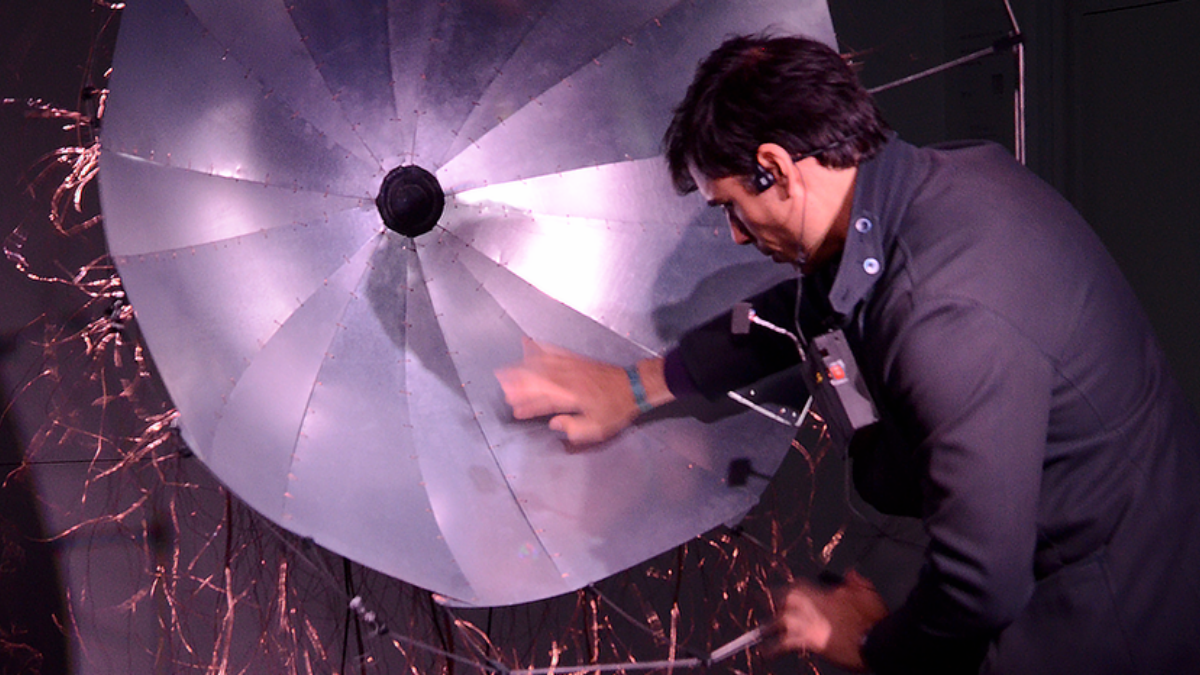
\includegraphics[width=0.45\linewidth]{c_2/chevalier18_1.png}}
    \hfill
    \subcaptionbox{Bloom: Space\label{fig: collaborativeARt-bloom}}{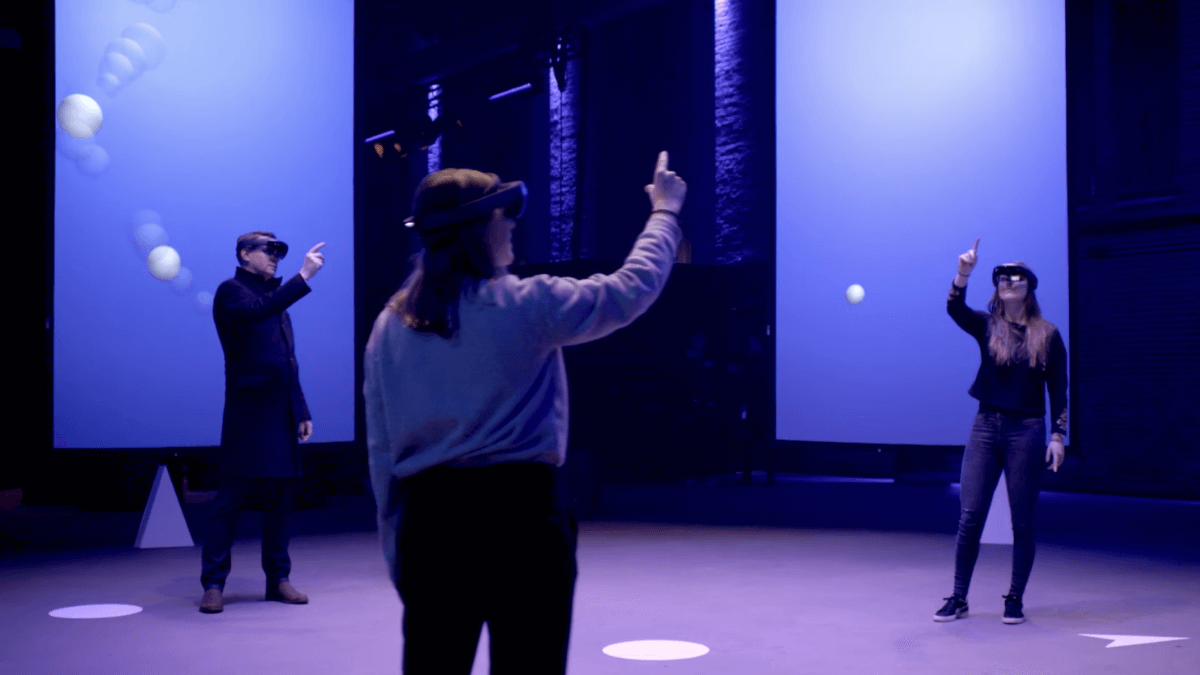
\includegraphics[width=0.45\linewidth]{c_2/bloom.png}}
    \caption{Collaborative Expression in AR}
    \label{fig: collaborativeARt}
\end{figure}

\subsection{Activism and Agency}\label{sec: literature-arts-activism}
Due to its ability to be an effective tool for collaborative expression, or perhaps because it creates a liminal hybridity that `questions the possession and control of a physical space' \citep{thiel2018}, AR art has seen use in activism and collaborative political expression. Early pioneers such as the Manifest.AR group were able to create convincing and socially immersive AR art using visual layering \footnote{\url{http://www.sndrv.nl/moma/}}. They did this through aligning the collaborative potential of AR with political expression. By creating an app that overlaid visual art within the Museum of Modern Art (MoMA) through GPS, they allowed participants to visit an exhibition in the museum that had not been organised by MoMA themselves (\autoref{fig: activismARt-moma}). AR thereby afforded these artists the ability to embed virtual art within an area considered private property, and also promote collective AR agency, raising very early questions about `virtual trespass' with AR. In a similar vein, `\#arOCCUPYWALLSTREET' (\#arOWS) was an arm of the Occupy Wall Street protests of 2011. Some 25 artists succeeded in overlaying the Wall Street area with `over 400 protest related augments', including audio overlays of protesters who were forbidden by police to enter the area. In this way, `AR was able to overcome their surveillance, barricades, horses, and excessive police numbers' \citeyearpar{skwarek2018} and more easily provide the means to action to people unable to physically mobilise.

As well as its liminality between real and virtual space promoting otherwise dangerous collaborative expression, AR has the power of rendering the invisible as seen, and due to this, it is a tool that has be used to shine light on social, economic, political and environmental injustices. Through its ability to change our perception of the real world through sensory augmentation, diminishment, hybridisation and extension, it has been used as a medium within the arts to `uncover' underlying mechanisms in our society. For example, Thiel and PATTU's (artists Cem Kozar and Işıl Ünal) 2011 work `Invisible Istanbul' aims to render visible the unseen urban dynamics of Istanbul, through GPS positioning smartphone visual overlay. They write: `Viewers become as photographers: the act of viewing or making a screenshot of the objects at a specific site and time reifies the virtual objects into artworks, revealing hidden forces within the city not visible to the naked eye.' \citeyearpar{thiel2011}. In PATTU's work, an augmented reality walking tour, different parts of the city are overlaid with symbolic information of past, present, and future uses of each area, highlighting tensions from military and commercial uses, and the effects this has on `contemporary urban space and the lives of its inhabitants' \citeyearpar{thiel2018}.

\begin{figure}
    \centering
    \subcaptionbox{Manifest.AR MoMA Invasion\label{fig: activismARt-moma}}{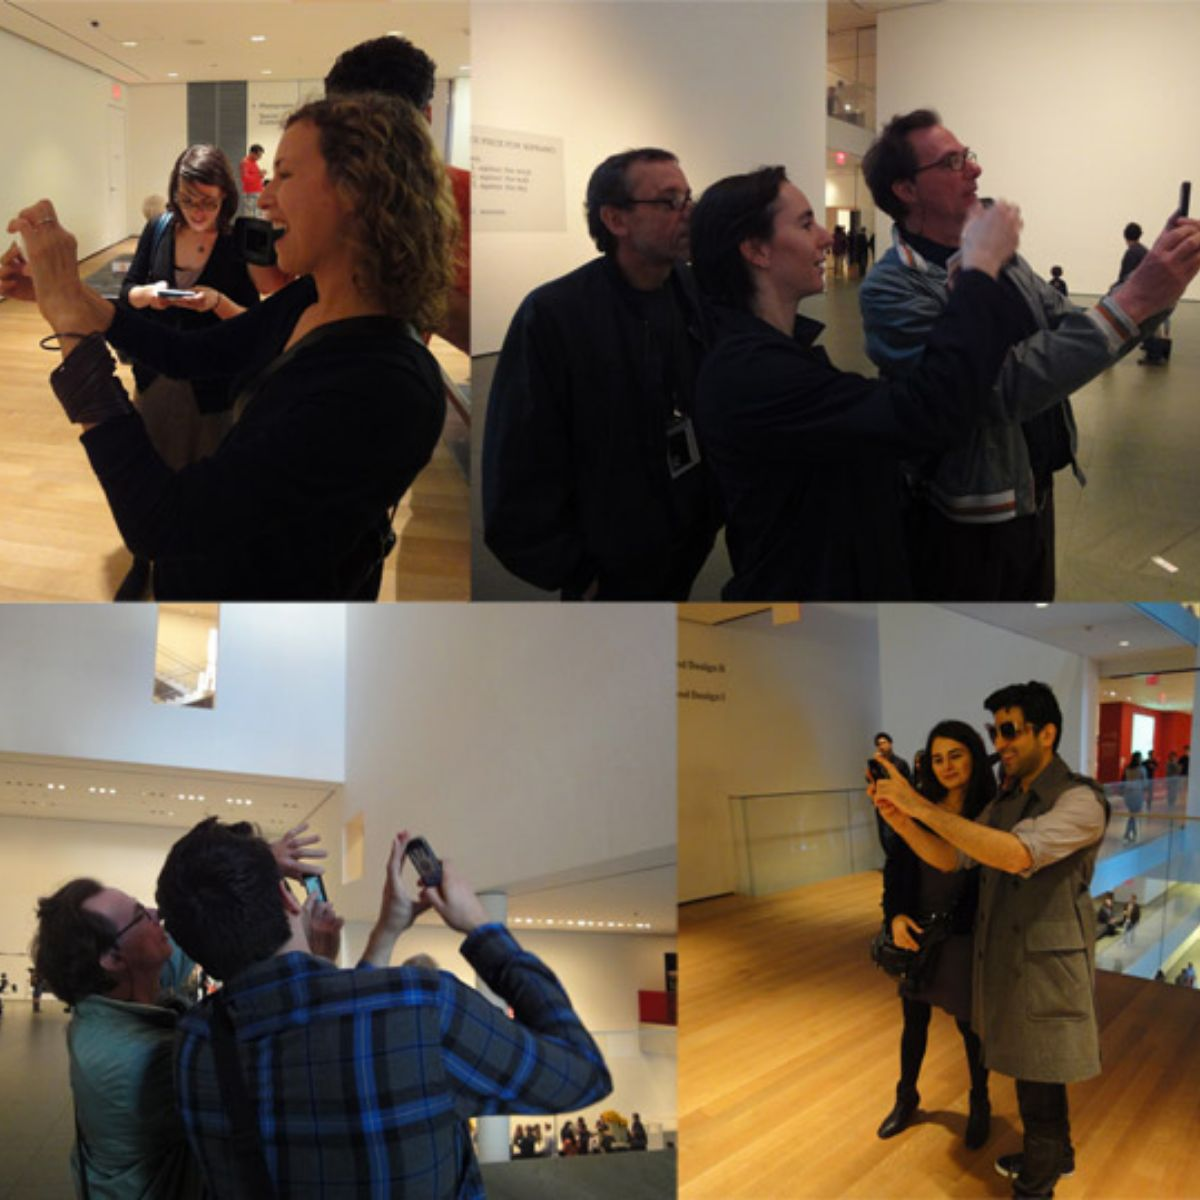
\includegraphics[width=0.45\linewidth]{c_2/moma.jpg}}
    \hfill
    \subcaptionbox{Invisible Istanbul\label{fig: activismARt-istanbul}}{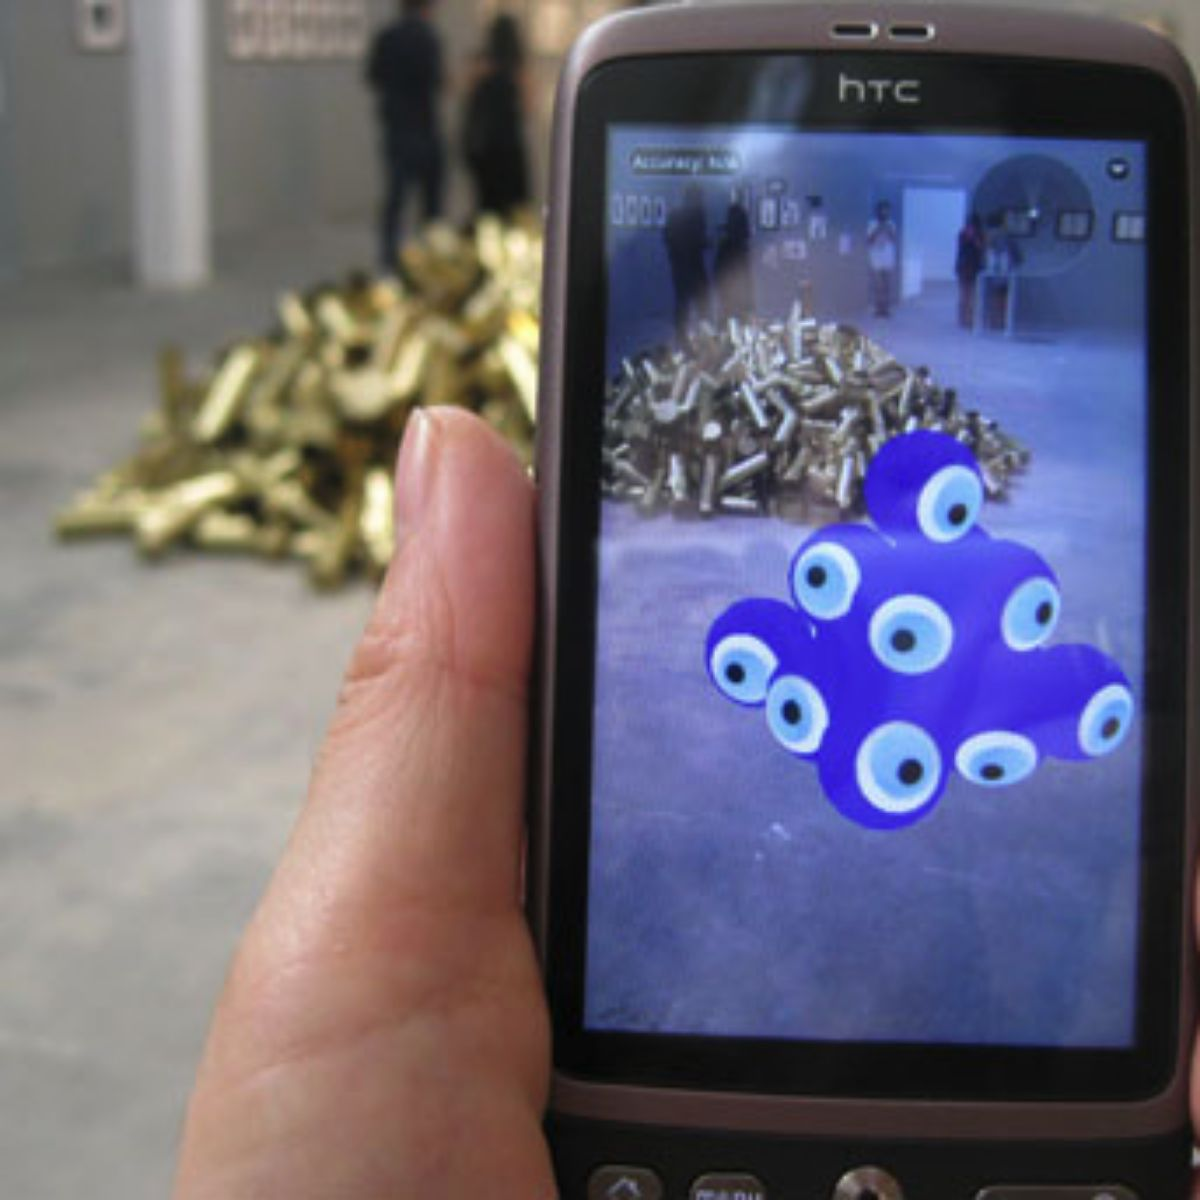
\includegraphics[width=0.45\linewidth]{c_2/thiel.jpg}}
    \caption{Activism through Interventionist ARt}
    \label{fig: activismARt}
\end{figure}

As summarised by Manifest.AR member Martin Skwarek puts it: `Alice has stepped through the looking glass [...] It is the job all future artists and activists to use this technology for the better, to bring people together, and uproot social injustice.' \citeyearpar{skwarek2018}



\subsection{An Arts Approach to Designing Multisensory AR}\label{sec: literature-arts-designingart}
Agreeing that AR can be used as a medium for the composition of computational art through software tool or instrument design, surfaces the question of what the materiality, both for user and developer, of such a digital tool, or piece software would look, sound, feel, taste or smell like. As Papagiannis highlights, `Understanding the capacities of the technology and its constraints to exploit the technology to artistic use by envisioning novel applications and approaches, and developing new aesthetics and conventions beyond previous traditional forms' \citeyearpar{papagiannis2017}.

If visual overlay AR has been used as `a viewing instrument to bring into focus forces invisible to the naked or unknowing eye, and make them visible in the public sphere.' \citep{thiel2011}, what emergent properties might devices rising out from multisensory approaches to design afford? What are the futures of digital musical instruments, whos designers opt to use this technology?

The next chapter explores three theoretical approaches that will help us understand more about the hybrid real-virtual \emph{space} it co-constructs with participants when in use, the \emph{materiality} afforded by AR when used as a medium for creative expression, and the experience of \emph{embodiment} it has the potential of imparting on these participants.
